\section{System Overview}
\label{sec:System_Overview}
The aggregate system is shown in Figure \ref{fig:sys_overview} and consists of a manipulator, a gripper, an object, a tracking system, control computers, a fluidic drive array and a rigid frame.
The planar six segment soft rubber manipulator consists of twelve distributed elastomer actuators. This manipulator moves with minimal friction on a level plane.
A soft rubber gripper is fixed to the tip of the manipulator.
An object is randomly placed within the reachable envelop of the manipulator. 
A motion capture system provides real-time measurements of marked points both along the inextensible back of the manipulator and on top of the object. 
The grasp motion planning algorithm as well as the curvature controller run on the control computers and take the tracking information as input.
The curvature controller then provides continuous closed-loop adjustment of the fluidic drive cylinder array.
The cylinder array directly actuates the manipulator and gripper.
A rigid frame holds all the subsystems together providing reliable and consistent hardware experiments.

\begin{figure}[htbp]
\begin{centering}
  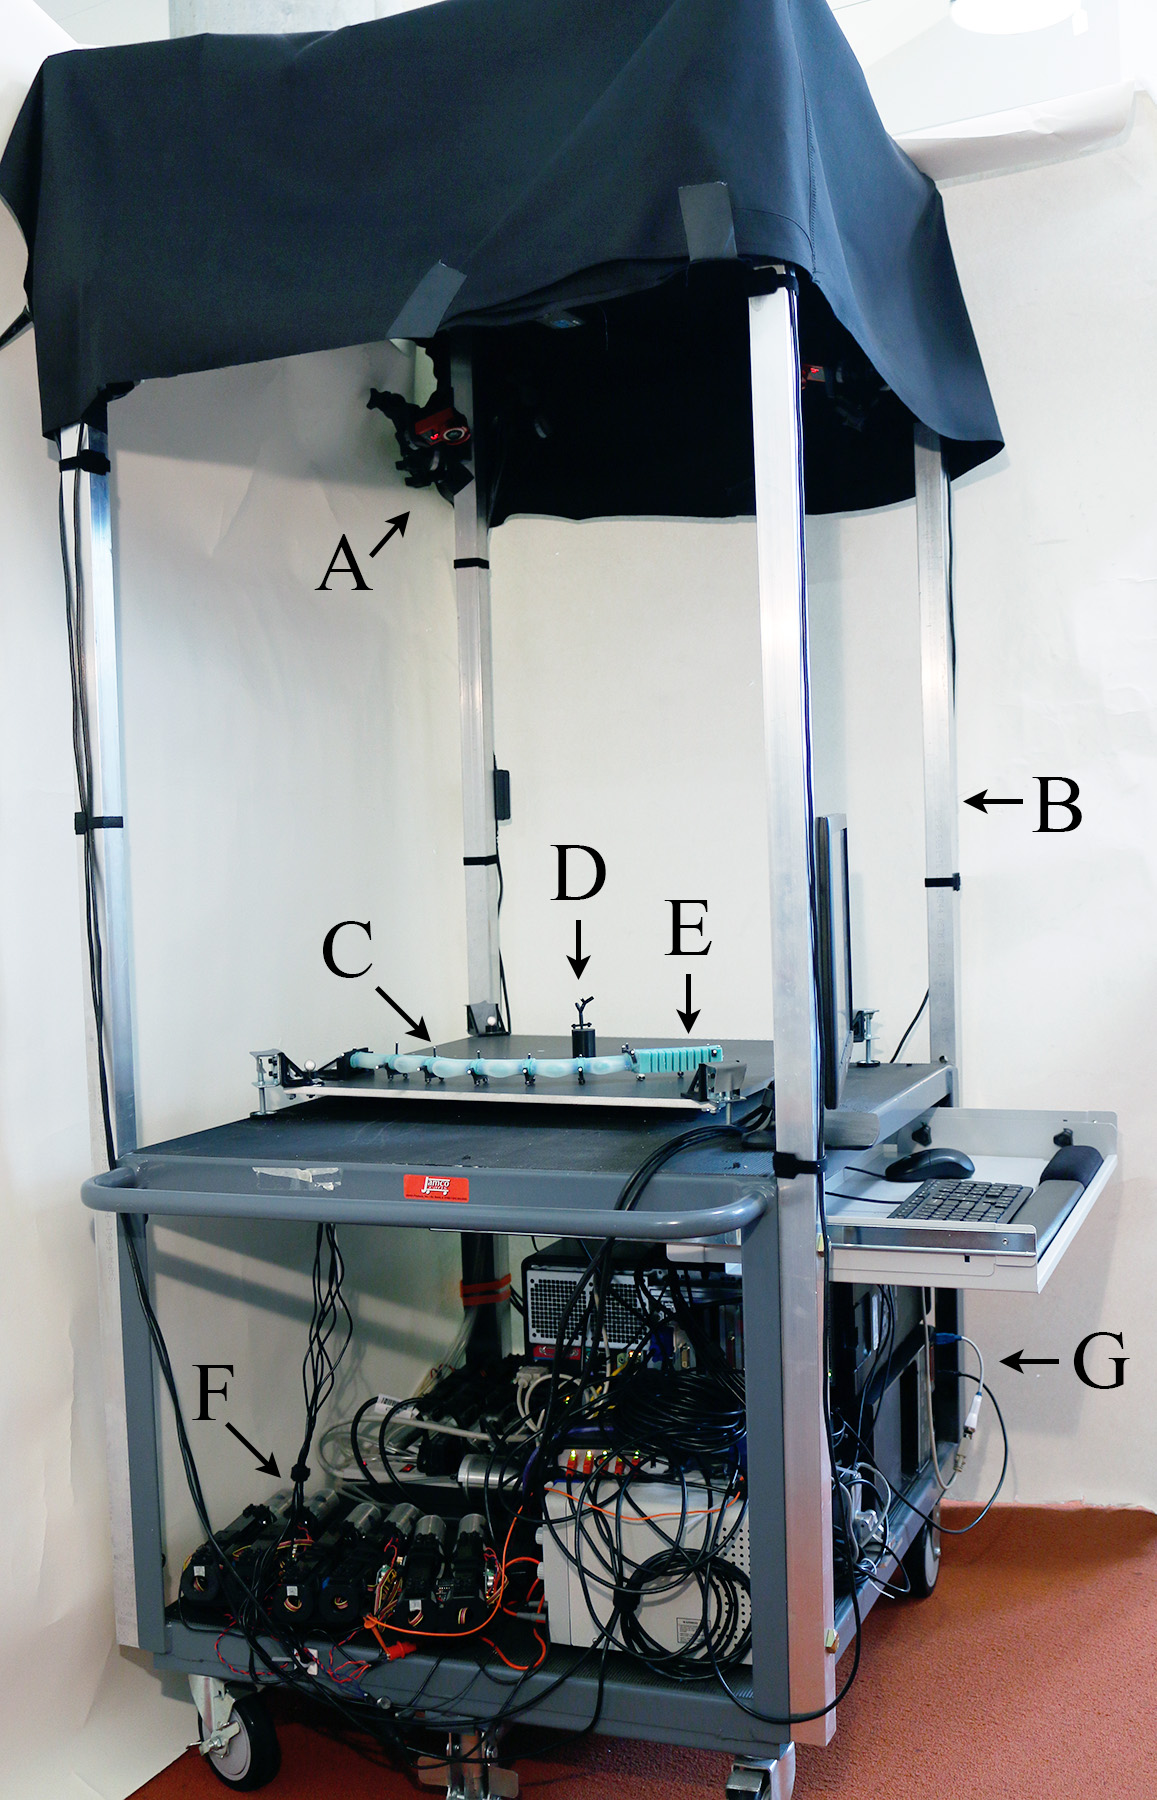
\includegraphics[width=2.0in]{Figures/system_overview/sys_overview_smaller}\\
  \caption{System Overview. The system is composed of a motion capture system (A), rigid frame (B), soft six segment planar manipulator (C), an object within the grasp envelope (D), a soft gripper fixed to the manipulator (E), a fluidic drive cylinder array to control actuation (F), and computers for real-time processing and control (G).} \label{fig:sys_overview}
\end{centering}
\end{figure}
